\section{Pressione Oncotica}
La parete dei capillari del sangue è costituita da tessuto epiteliale con spessore di qualche $\mu m$. Tale parete separa il sangue dal liquido interstiziale e si comporta come una membrana semipermeabile: è infatti permeabile agli ioni e in generale ai \textit{cristalloidi}, e impermeabile ai \textit{colloidi} come le proteine.\footnote{i \textit{cristalloidi} sono sostanze facilmente diffondibili attraverso la membrana endoteliale e comprendono ioni e composti a basso peso molecolare come sodio e glucosio; i \textit{colloidi} sono sostanze non solvatate e ad alto peso molecolare non diffondibili attraverso l'endotelio.}
Fra il plasma nei capillari e il liquido interstiziale esiste pertanto una differenza di pressione osmotica determinata dalla presenza delle proteine nel plasma e dalla loro (quasi) assenza nell'interstizio. La pressione osmotica derivante dalla sola componente proteica viene chiamata pressione \textit{oncotica}, oppure \textit{colloido-osmotica}.

Affinché vi sia equilibrio dinamico tra plasma e liquido interstiziale, è necessario che la differenza di pressione osmotica tra i due compartimenti sia annullata da una differenza di pressione idraulica. La situazione, basata sull'\textit{ipotesi di Starling}, è illustrata in \figurename~\ref{starling}.
\begin{figure}[htb]
	\centering
	\subfigure[]%
	{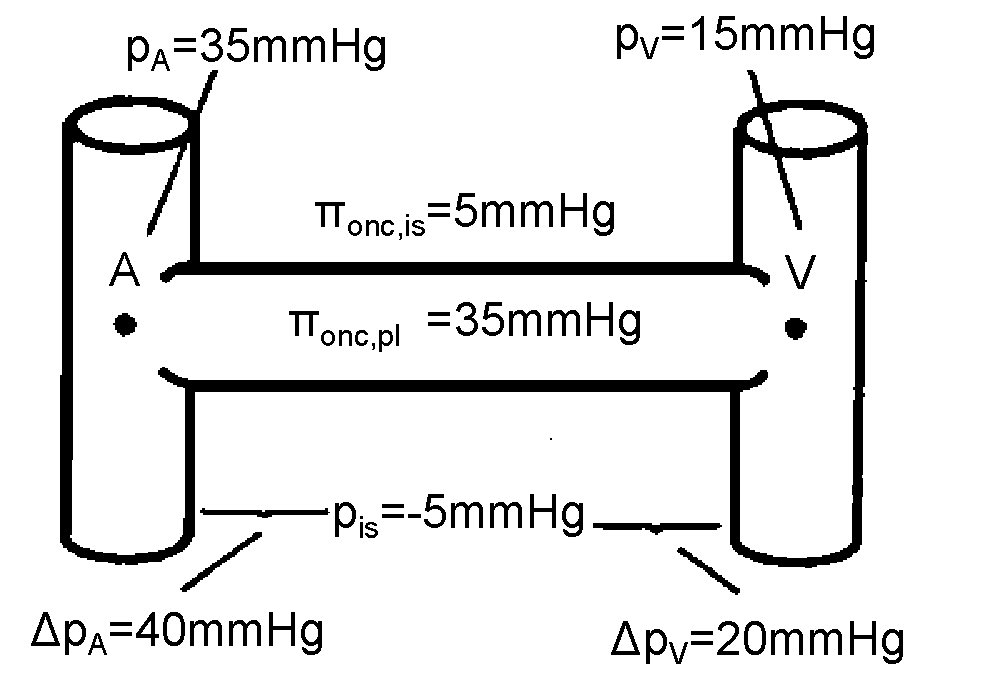
\includegraphics[width=0.30\textwidth]{immagini/starling1.eps}}
	\subfigure[]%
	{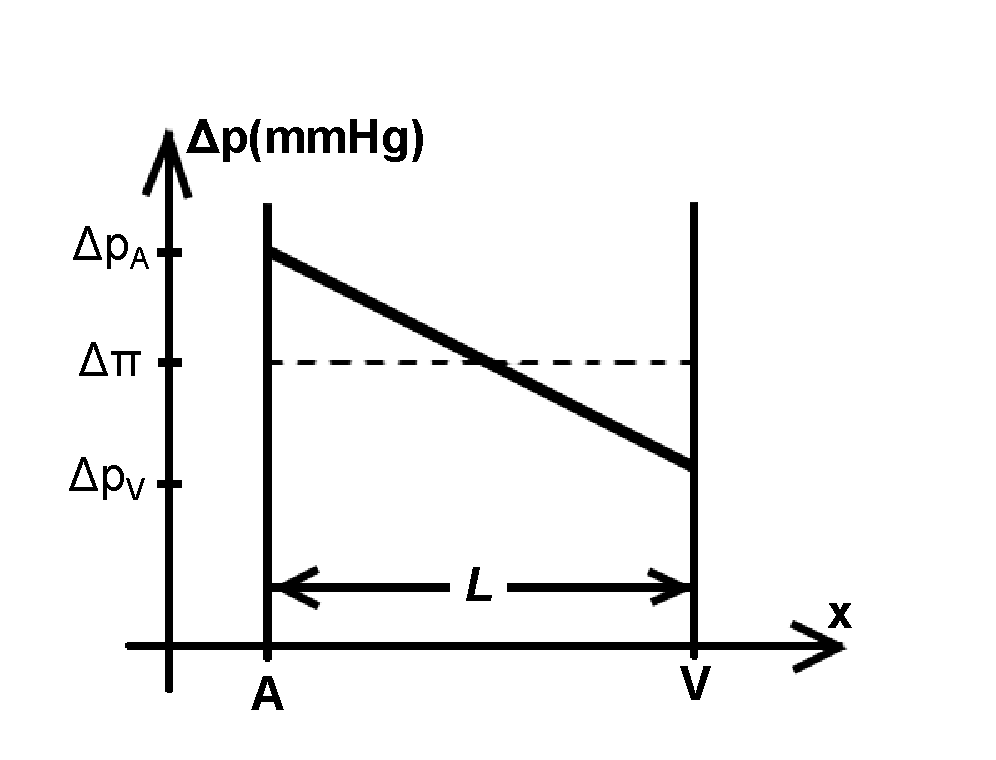
\includegraphics[width=0.35\textwidth]{immagini/starling2.eps}}
	\subfigure[]%
	{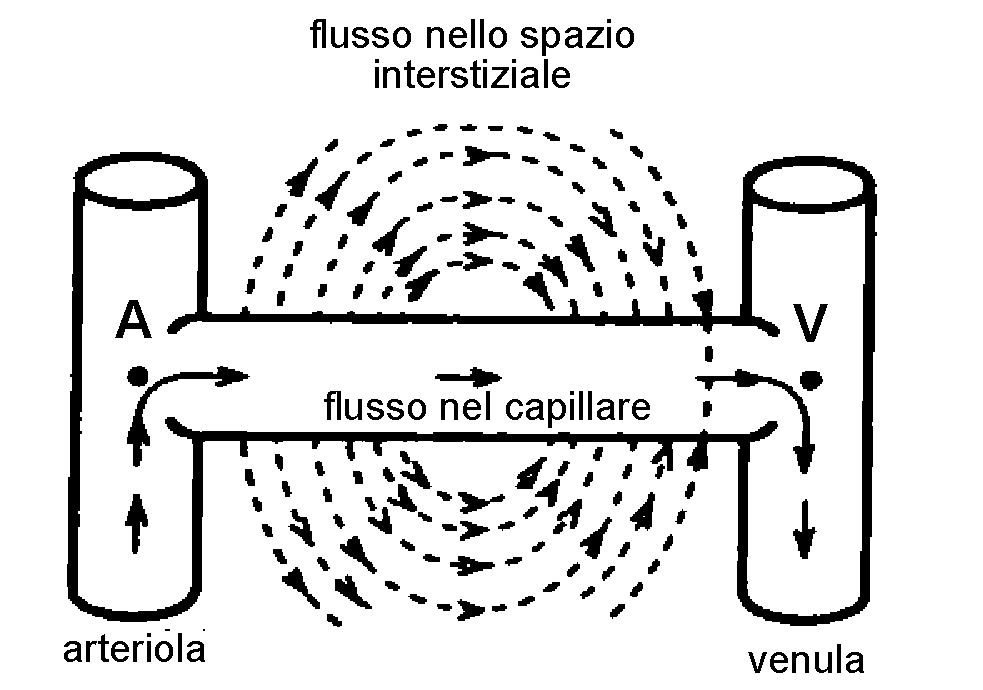
\includegraphics[width=0.30\textwidth]{immagini/starling3.eps}}
		\caption{Ipotesi di \textit{Starling}: lungo il capillare la pressione idraulica diminuisce mentre quella osmotica dovuta alle proteine resta costante in modo che si verifichi una microcircolazione locale a flusso netto nullo.}\label{starling}
\end{figure}
\noindent
In media non vi è flusso netto di fluidi in entrata o in uscita dal capillare, ma poiché la pressione attraverso la parete non è costante lungo il capillare, vi sarà un flusso localizzato di fluidi in uscita dal capillare all'estremità arteriosa e in ingresso al capillare all'estremità venosa, tale però da annullare il flusso complessivo lungo tutto il capillare.
In questo modo si verifica una \textit{microcircolazione}\footnote{un'alterazione della permeabilità della membrana, provocata ad esempio da uno stato infiammatorio, può causare uno sbilanciamento della microcircolazione con conseguente \textit{edema}.} attorno al capillare, consentendo il trasferimento di sostanze nutritive verso i tessuti e il richiamo di sostanze di scarto dai tessuti al sangue.
Se si provasse a calcolare la pressione oncotica con la formula di \textit{Van't Hoff} $$\Pi=\delta \frac{nRT}{V}$$ si troverebbero dei valori molto diversi rispetto a quelli fisiologici. Il divario è dovuto al fatto che le proteine non sono neutre ma, a $pH$ fisiologico, si trovano in forma anionica e tendono a influenzare la diffusibilità, e quindi l'effetto osmotico, delle altre molecole elettricamente cariche. Per calcolare la pressione oncotica, sia nel compartimento plasmatico che in quello interstiziale, si è utilizzata le seguente equazione di \textit{Landis-Pappenheimer} \cite{original_L-P, corrected_L-P}:
\begin{equation}
	\Pi_{onc} = 2.1\cdot T_p + 0.16\cdot T_p^2 + 0.009\cdot T_p^3
	\label{LPpl}
\end{equation}
che restituisce valori in $mmHg$ se la concentrazione delle proteine totali $T_p$ è espressa in $gr/dL$.
Considerando che all'equilibrio le proteine totali plasmatiche sono circa pari a $7$ $gr/dL$ e che le proteine interstiziali sono un sesto di quelle plasmatiche \cite{guyton}, la differenza di pressione osmotica fra plasma e interstizio risulta pari a circa:
$$\Pi_{onc}(7)-\Pi_{onc}(7/6)=23\text{ }mmHg$$
